\let\negmedspace\undefined
\let\negthickspace\undefined
\documentclass[journal,12pt,twocolumn]{IEEEtran}
\usepackage{cite}
\usepackage{amsmath,amssymb,amsfonts,amsthm}
\usepackage{algorithmic}
\usepackage{graphicx}
\usepackage{textcomp}
\usepackage{xcolor}
\usepackage{txfonts}
\usepackage{listings}
\usepackage{enumitem}
\usepackage{mathtools}
\usepackage{gensymb}
\usepackage[breaklinks=true]{hyperref}
\usepackage{tkz-euclide} % loads  TikZ and tkz-base
\usepackage{listings}
\DeclareMathOperator*{\Res}{Res}
%\renewcommand{\baselinestretch}{2}
\renewcommand\thesection{\arabic{section}}
\renewcommand\thesubsection{\thesection.\arabic{subsection}}
\renewcommand\thesubsubsection{\thesubsection.\arabic{subsubsection}}
\renewcommand\thesectiondis{\arabic{section}}
\renewcommand\thesubsectiondis{\thesectiondis.\arabic{subsection}}
\renewcommand\thesubsubsectiondis{\thesubsectiondis.\arabic{subsubsection}}
% correct bad hyphenation here
\hyphenation{op-tical net-works semi-conduc-tor}
\def\inputGnumericTable{}                                 %%
% \lstset{
% %language&=C,
% frame&=single,
% breaklines&=true,
% columns&=fullflexible
% }
%\lstset{
%language&=tex,
%frame&=single, 
%breaklines&=true
%}

%


\newtheorem{theorem}{Theorem}[section]
\newtheorem{problem}{Problem}
\newtheorem{proposition}{Proposition}[section]
\newtheorem{lemma}{Lemma}[section]
\newtheorem{corollary}[theorem]{Corollary}
\newtheorem{example}{Example}[section]
\newtheorem{definition}[problem]{Definition}
%\newtheorem{thm}{Theorem}[section] 
%\newtheorem{defn}[thm]{Definition}
%\newtheorem{algorithm}{Algorithm}[section]
%\newtheorem{cor}{Corollary}
\newcommand{\BEQA}{\begin{eqnarray}}
\newcommand{\EEQA}{\end{eqnarray}}
\newcommand{\define}{\stackrel{\triangle}{&=}}

\bibliographystyle{IEEEtran}
\providecommand{\mbf}{}
\providecommand{\pr}[1]{\ensuremath{\Pr\left(#1\right)}}
\providecommand{\qfunc}[1]{\ensuremath{Q\left(#1\right)}}
\providecommand{\sbrak}[1]{\ensuremath{{}\left[#1\right]}}
\providecommand{\lsbrak}[1]{\ensuremath{{}\left[#1\right.}}
\providecommand{\rsbrak}[1]{\ensuremath{{}\left.#1\right]}}
\providecommand{\brak}[1]{\ensuremath{\left(#1\right)}}
\providecommand{\lbrak}[1]{\ensuremath{\left(#1\right.}}
\providecommand{\rbrak}[1]{\ensuremath{\left.#1\right)}}
\providecommand{\cbrak}[1]{\ensuremath{\left\{#1\right\}}}
\providecommand{\lcbrak}[1]{\ensuremath{\left\{#1\right.}}
\providecommand{\rcbrak}[1]{\ensuremath{\left.#1\right\}}}
\theoremstyle{remark}
\newtheorem{rem}{Remark}
\newcommand{\sgn}{\mathop{\mathrm{sgn}}}
\providecommand{\abs}[1]{$\left\vert#1\right\vert$}
\providecommand{\res}[1]{\Res\displaylimits_{#1}}
\providecommand{\norm}[1]{$\left\lVert#1\right\rVert$}
%\providecommand{\norm}[1]{\lVert#1\rVert}
\providecommand{\mtx}[1]{{#1}}
\providecommand{\mean}[1]{$E\left[ #1 \right]$}
\providecommand{\fourier}{\overset{\mathcal{F}}{ \rightleftharpoons}}
%\providecommand{\hilbert}{\overset{\mathcal{H}}{ \rightleftharpoons}}
\providecommand{\system}{\overset{\mathcal{H}}{ \longleftrightarrow}}
        %\newcommand{\solution}[2]{\textbf{Solution:}{#1}}
\newcommand{\solution}{\noindent \textbf{Solution: }}
\newcommand{\cosec}{\,\text{cosec}\,}
\providecommand{\dec}[2]{\ensuremath{\overset{#1}{\underset{#2}{\gtrless}}}}
\newcommand{\myvec}[1]{\ensuremath{\begin{pmatrix}#1\end{pmatrix}}}
\newcommand{\mydet}[1]{\ensuremath{\begin{vmatrix}#1\end{vmatrix}}}
\let\vec
%\renewcommand{\thefigure}{\theproblem.\arabic{figure}}
%\renewcommand{\thefigure}{\theproblem}
%\setlist[enumerate,1]{before&=\renewcommand\theequation{\theenumi.\arabic{equation}}
%\counterwithin{equation}{enumi}


%\renewcommand{\theequation}{\arabic{subsection}.\arabic{equation}}

%\def\putbox#1#2#3{\makebox[0in][l]{\makebox[#1][l]{}\raisebox{\baselineskip}[0in][0in]{\raisebox{#2}[0in][0in]{#3}}}}
%     \def\rightbox#1{\makebox[0in][r]{#1}}
%     \def\centbox#1{\makebox[0in]{#1}}
%     \def\topbox#1{\raisebox{-\baselineskip}[0in][0in]{#1}}
%     \def\midbox#1{\raisebox{-0.5\baselineskip}[0in][0in]{#1}}
\vspace{3cm}
\title{Probability Assignment}
\author{Advait Jain \\ (CS22BTECH11003)}


\usepackage{graphicx} % Required for inserting images

\begin{document}

\maketitle
\section*{Introduction}
Randomness is a fundamental component of many computer science applications, including simulations, cryptography, games, and statistical analysis. In this assignment, we delve into the implementation of a random number generator using a shift registers 

\section*{Components used}
\begin{table}[htbp]
	\label{tab:Hardware_Assignment}
	%%%%%%%%%%%%%%%%%%%%%%%%%%%%%%%%%%%%%%%%%%%%%%%%%%%%%%%%%%%%%%%%%%%%%%
%%                                                                  %%
%%  This is a LaTeX2e table fragment exported from Gnumeric.        %%
%%                                                                  %%
%%%%%%%%%%%%%%%%%%%%%%%%%%%%%%%%%%%%%%%%%%%%%%%%%%%%%%%%%%%%%%%%%%%%%%
\begin{tabular}{|l|l|l|}\hline
	Component	&Value &Quantity\\ \hline
	Breadboard & &1 \\ \hline
	Seven Segment Diplay &Common Anode &1 \\ \hline
	Decoder &7447 &1 \\ \hline
	Flip Flop &7474 &2 \\ \hline
	X-OR Gate &7486 &1 \\ \hline
	555 IC & &1 \\ \hline
	Resistor &1 K$\Omega$ &1 \\ \hline
	Capacitor &100 nF &1 \\ \hline
	Capacitor &10 nF &1 \\ \hline
	Jumper Wires & & \\ \hline
\end{tabular}
\end{table}



\section*{Procedure}
\begin{enumerate}
	\item We connected the 555 timer circuit based on the following figure:
	\begin{figure}[h]
		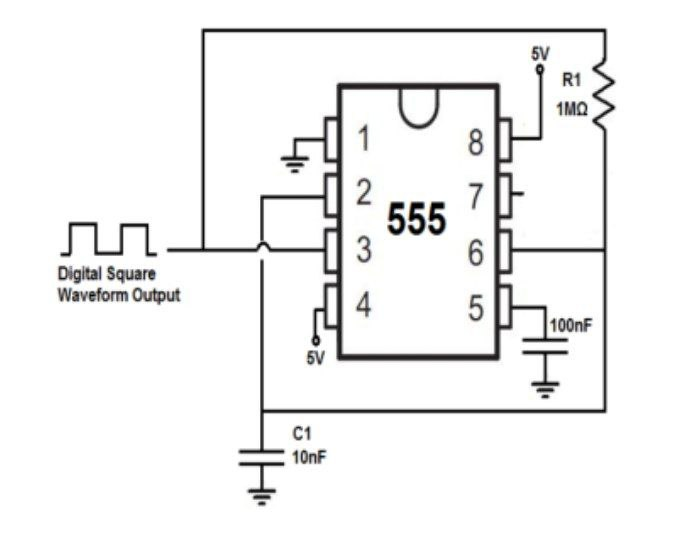
\includegraphics[width=\linewidth]{images/555_timer_circuit.jpg}
		\caption{Connection in 555 timer circuit}
		\label{555_t_c}
	\end{figure}
	
	\item Then, we connected the 555 timer's clock output to the D-flip flops' clock signal.
	
	\item Now we construct the shift register circuit that use four D-flip flops(7474 IC's).
	\begin{figure}[h]
		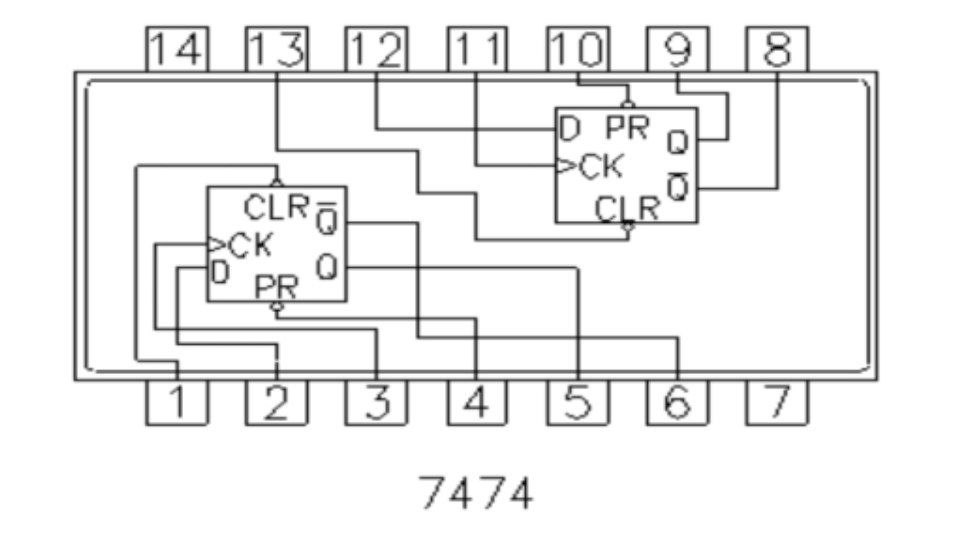
\includegraphics[width=\linewidth]{images/7474.jpg}
		\caption{Connection in 7474 IC}
		\label{7474_IC}
	\end{figure}

	\item Then, consistent with the diagram, we join the XOR gate (7486 IC).
	\begin{figure}[h]
		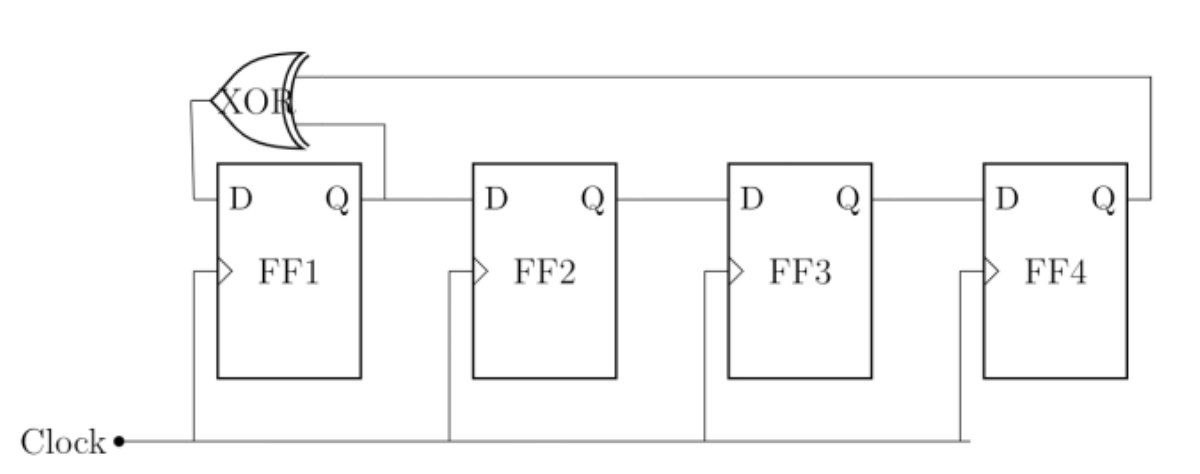
\includegraphics[width=\linewidth]{images/circuit_connections.jpg}
		\caption{Connection in XOR gate}
		\label{XOR}
	\end{figure}

	\item Following that, we joined the decoder (7447 IC), connecting its A, B, C, and D to $Q_0$, $Q_1$, $Q_2$, and $Q_3$, respectively, shown later in the diagram.
	\begin{figure}[h]
		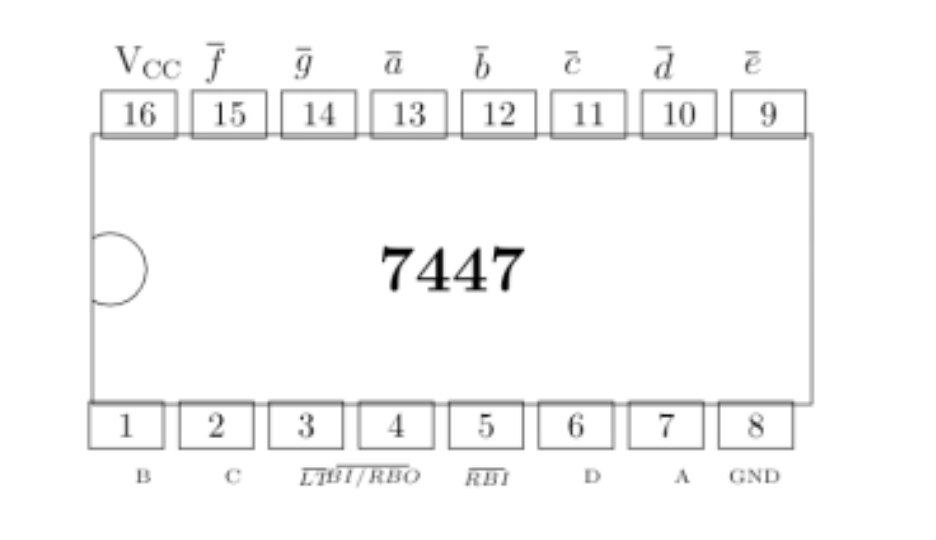
\includegraphics[width=\linewidth]{images/7447.jpg}
		\caption{Connection in Decoder gate}
  \label{7447}
	\end{figure}
		
	\item Then we connected The seven segmented display and connected it with the decoder (7447 IC) according to the table \ref{table} and the figure \ref{SSD}
	\begin{figure}[h]
		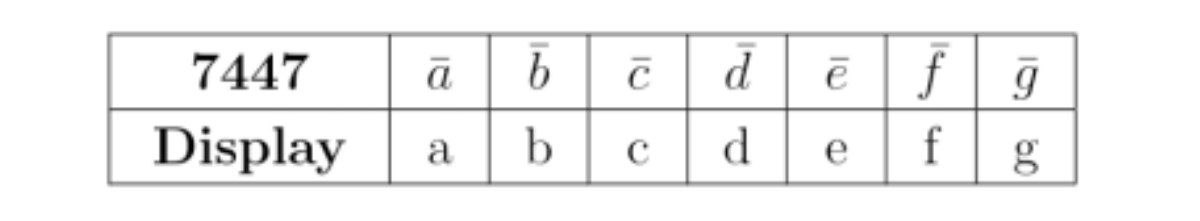
\includegraphics[width=\linewidth]{images/7447_table.jpg}
		\caption{Connection of seven segmented display with decoder}
		\label{table}
	\end{figure}
	\begin{figure}[h]
		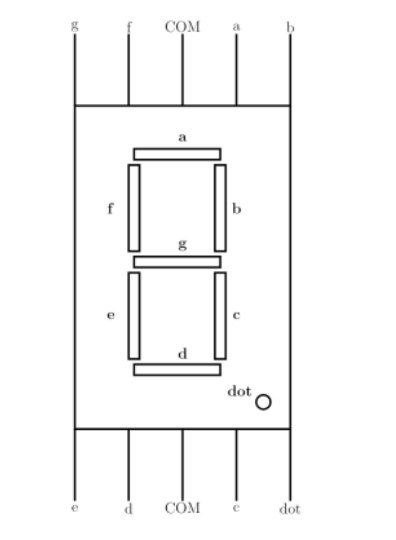
\includegraphics[width=\linewidth]{images/seven_segment_display.jpg}
		\caption{Seven segmented display}
		\label{SSD}
	\end{figure}

	\item Before connecting the power supply, we linked all of the independent components.
	
	
\section*{Output} 
	The seven segment display showed random numbers being generated continuously as the output.
	\begin{figure}[h]
		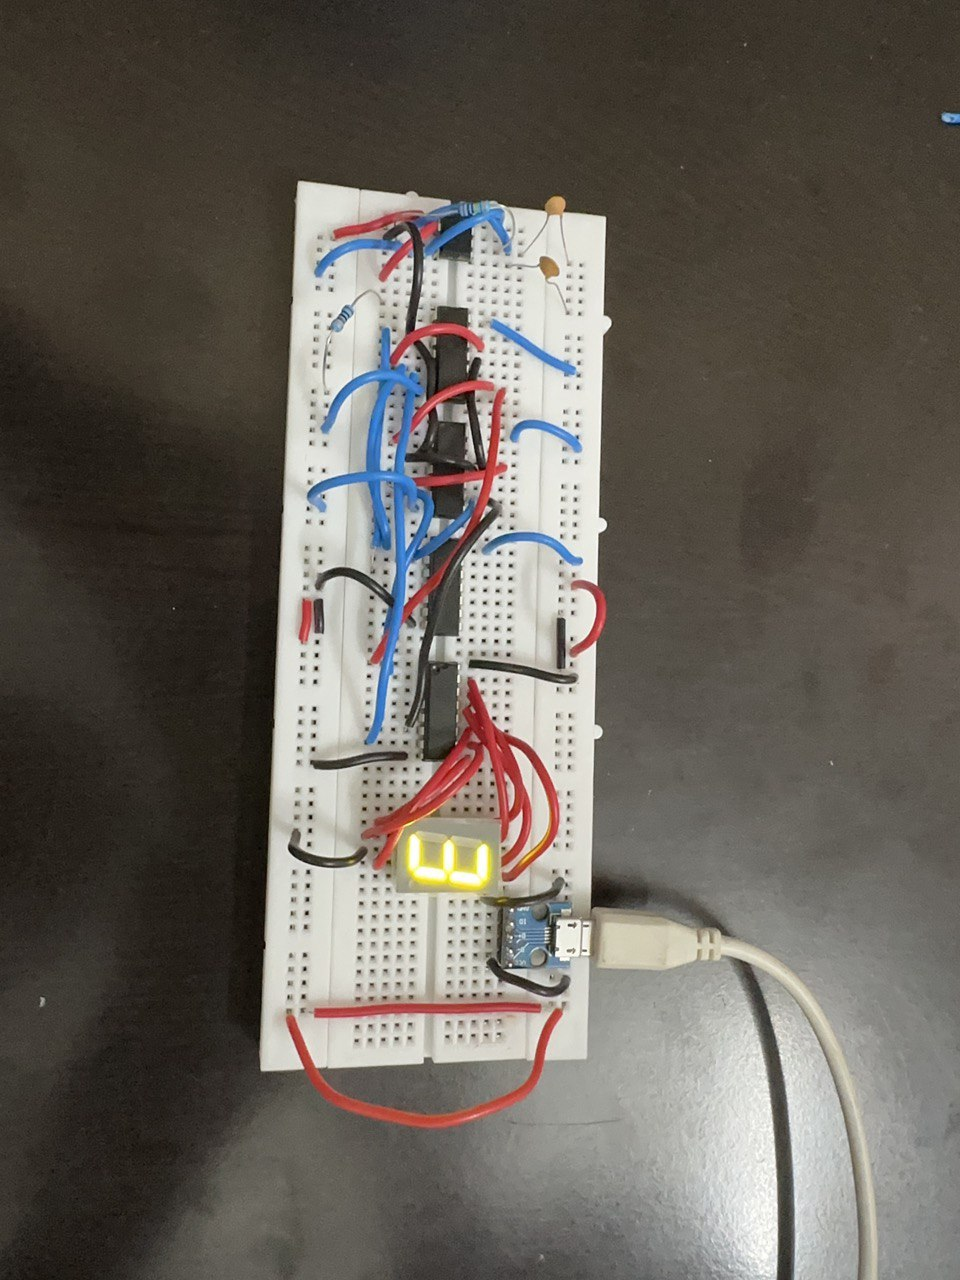
\includegraphics[width=0.3\linewidth]{images/output3.jpeg}
		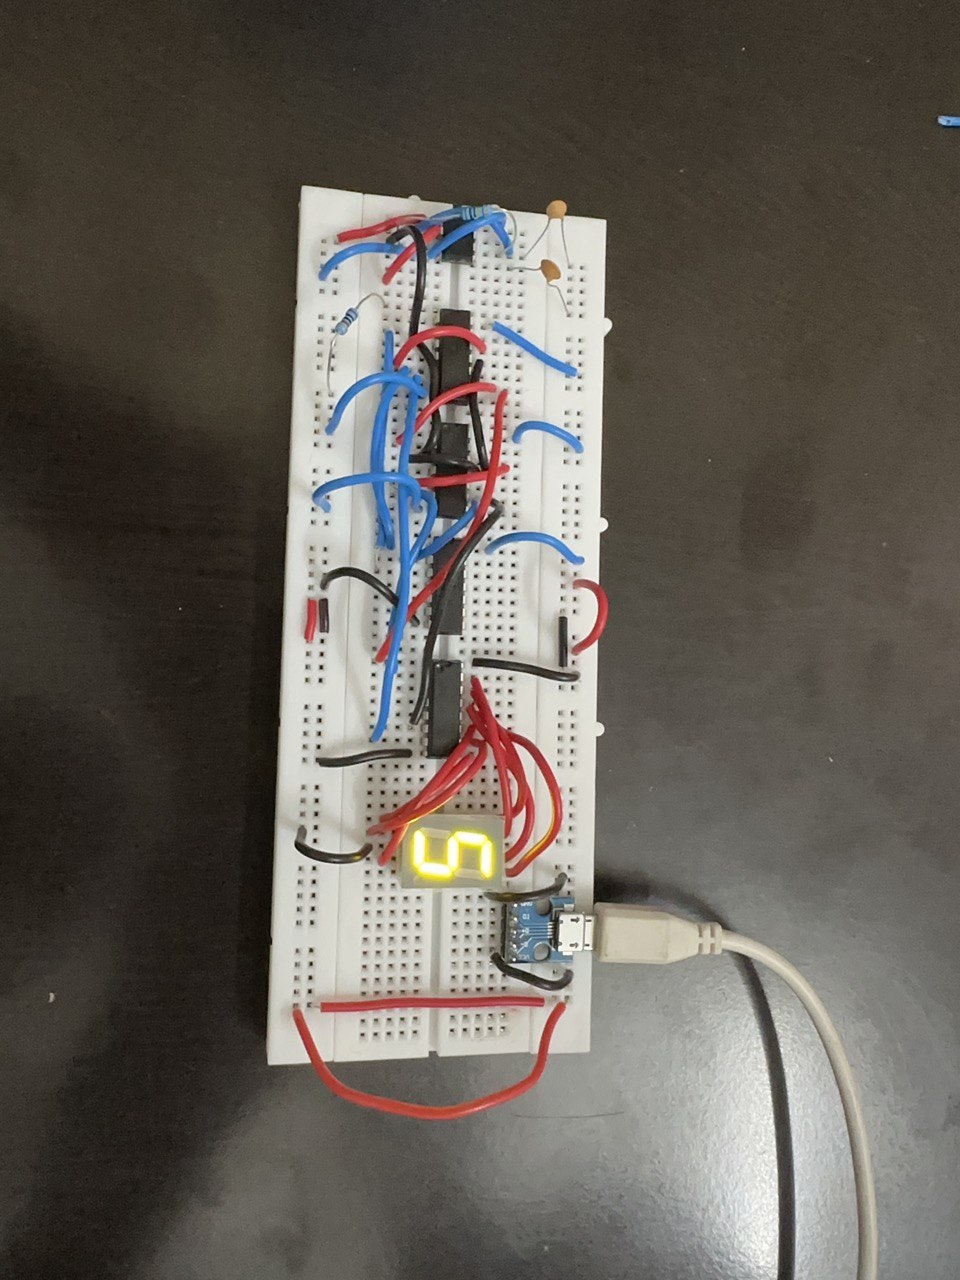
\includegraphics[width=0.3\linewidth]{images/output5.jpeg}
		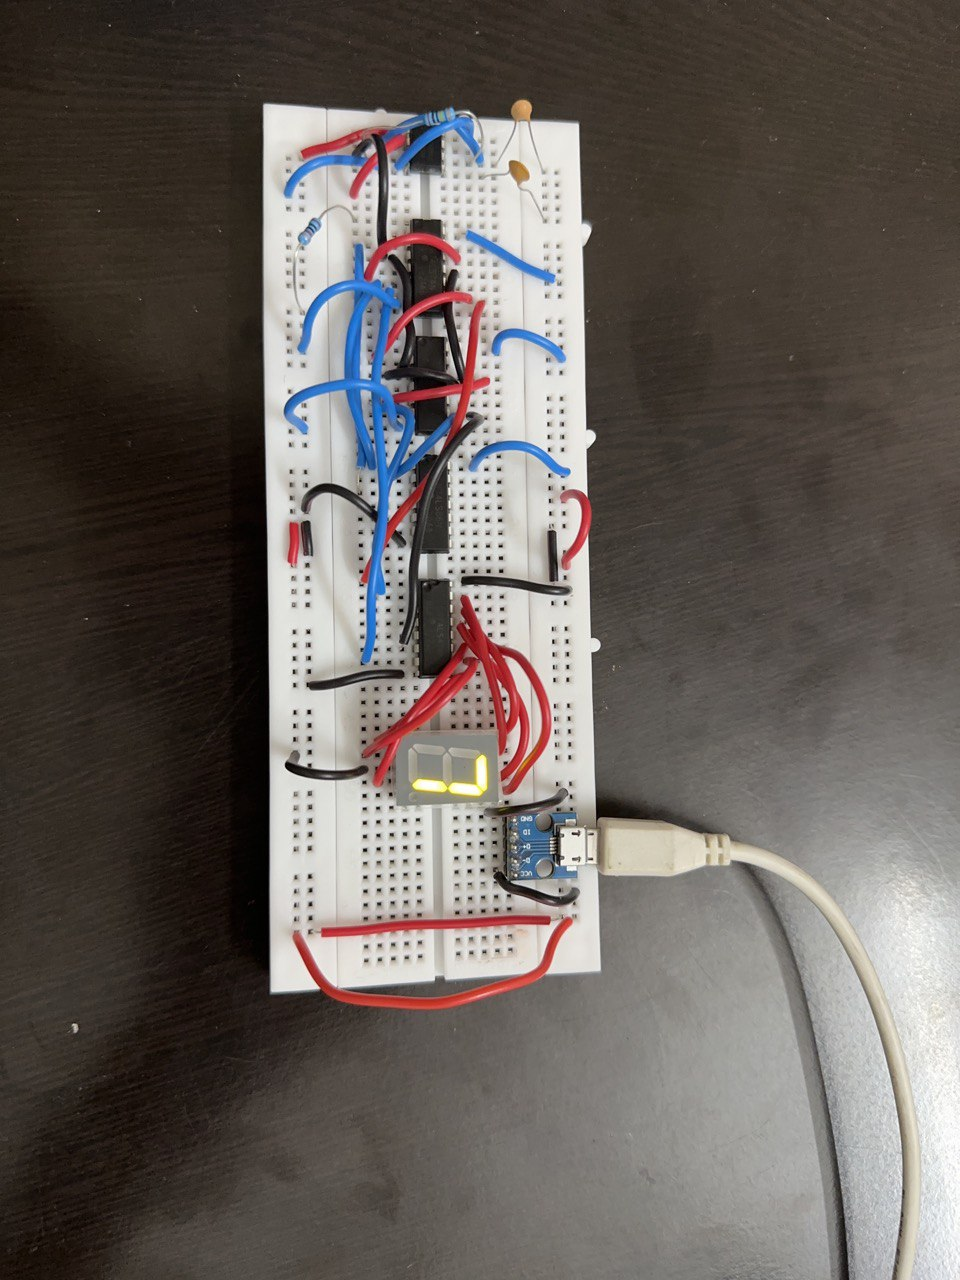
\includegraphics[width=0.3\linewidth]{images/output7.jpeg}
		\caption{Output}
		\label{SSD}
	\end{figure}
\end{enumerate}
\end{document}


